\documentclass[12pt,a4paper]{article}

\usepackage[margin=1in]{geometry}
\usepackage{graphicx}
\usepackage{amsmath}
\usepackage{booktabs}
\usepackage{float}
\usepackage{array}
\usepackage{longtable}
\usepackage{setspace}
\usepackage{hyperref}
\usepackage{titlesec}

\setstretch{1.15}
\setlength{\parskip}{0.5em}
\setlength{\parindent}{0pt}
\hypersetup{colorlinks=true,linkcolor=black,urlcolor=blue,citecolor=black}

\titleformat{\section}{\large\bfseries}{\thesection.}{0.5em}{}
\titleformat{\subsection}{\normalsize\bfseries}{\thesubsection}{0.5em}{}

\begin{document}

\begin{titlepage}
\centering

{\Large \textbf{Simulation-Based Implementation of Lean Manufacturing Techniques for Productivity Improvement:}}\\[0.3cm]
{\Large \textbf{A Data-Driven Case Study From a Beverage Bottling Line}}\\[1.2cm]

{\large \textbf{Final Research Paper}}\\[1cm]

\begin{tabular}{>{\bfseries}p{4.2cm}p{9.5cm}}
Submitted by & Divash Krishnam \\
Team Members & Ashutosh Verma, Raja \\
Department & Production and Industrial Engineering \\
Guided by & Dr.\ MOHD SHUAIB \\
Guide Department & Mechanical Department \\
\end{tabular}

\vfill

{\large Department of Production and Industrial Engineering}\\[0.2cm]
{\large Under the Guidance of Dr.\ MOHD SHUAIB, Mechanical Department}\\[0.8cm]
{\large \today}

\end{titlepage}

\tableofcontents
\newpage

\section*{Abstract}
Lean manufacturing is widely recognized as a practical and effective strategy for improving productivity, reducing waste, and stabilizing production flow. However, many small and medium-sized industries still face difficulty in identifying which lean tools should be implemented first, especially when resources are limited and repeated experimentation on the shop floor is risky. This study develops a self-contained, data-driven research framework for evaluating lean interventions using a real industrial production dataset from a beverage bottling line monitored through an Industrial Internet of Things (IIoT) system. The dataset contains 59 production summary records across 56 calendar production days between July 22, 2022 and February 6, 2023, 265 hourly operating observations, and 1,388 downtime events. The study first analyzes the production system through throughput, operating time, pause time, product mix, and temporal efficiency variation. Next, the downtime structure is examined by classifying events into micro-, minor-, and major-stoppage categories. Finally, an event-level bootstrap simulation is used to compare three lean scenarios: 5S with visual management, total productive maintenance (TPM), and an integrated lean bundle. The observed system produced 212,358 liters with an overall availability of 42.66\%. Downtime analysis shows that micro-stoppages represent 61.31\% of all events but only 13.59\% of total downtime minutes, whereas major stoppages represent only 6.77\% of events but consume 66.26\% of lost time. Simulation results show that 5S and visual management improve output by 2.33\%, TPM improves output by 20.61\%, and the integrated lean bundle improves output by 32.19\%, while increasing simulated availability from 42.37\% to 55.33\%. The main implication is that maintenance-led reduction of major stoppages should be prioritized before broader workplace-organization efforts when downtime severity is highly concentrated. The study contributes a reproducible open-data framework for simulation-based lean analysis and provides a complete final-year research-paper template for manufacturing engineering students.

\section*{Keywords}
Lean manufacturing, productivity improvement, small-scale industries, discrete-event simulation, beverage bottling line, downtime analysis, total productive maintenance, 5S, IIoT, digital manufacturing.

\newpage
\section{Introduction}
Lean manufacturing has become one of the most influential improvement philosophies in industrial engineering because it focuses on eliminating waste, improving flow, increasing responsiveness, and enhancing process discipline. In practice, however, lean implementation is rarely straightforward. Many organizations, especially smaller firms, understand the value of lean at a conceptual level but struggle to determine which tools should be applied first and where the highest-impact waste actually exists.

For small-scale industries and SMEs, this decision is especially important. Such firms often operate with constrained budgets, limited technical manpower, and less tolerance for failed improvement initiatives. If a company selects the wrong improvement priority, it may spend time and effort without producing meaningful productivity gains. For this reason, simulation-based lean implementation is highly valuable. It allows researchers and managers to test alternative interventions in a virtual decision environment before changing the real production system.

The topic originally considered for this work was \textit{Simulation-Based Implementation of Lean Manufacturing Techniques for Productivity Improvement in Small-Scale Industries}. That topic remains highly relevant, but the present paper refines it into a stronger research design by using a real open industrial dataset instead of hypothetical or purely conceptual examples. The use of real production and downtime data makes the analysis more rigorous, reproducible, and suitable for final-year academic work.

The present study uses an open dataset from a beverage bottling line that was monitored through IIoT infrastructure. This is particularly useful because the dataset includes production output, operating time, and detailed downtime-event logs, allowing a direct connection between shop-floor losses and lean scenario design. Instead of merely describing lean concepts, the paper quantitatively tests which lean interventions would provide the highest productivity improvement.

The broad motivation for the study is therefore twofold. First, it aims to demonstrate how lean manufacturing can be evaluated scientifically through real production data and simulation. Second, it aims to offer a practical model that students and SME practitioners can adapt for similar production systems.

The main objectives of this study are:
\begin{enumerate}
    \item to analyze the production behavior and downtime structure of a real bottling-line system;
    \item to identify the dominant operational waste pattern affecting productivity;
    \item to simulate the productivity impact of selected lean interventions; and
    \item to recommend an implementation priority for lean techniques based on data-driven evidence.
\end{enumerate}

\section{Literature Review and Research Gap}
Lean manufacturing has long been associated with better operational performance, especially in terms of productivity, quality, throughput, and waste reduction. Belekoukias \emph{et al.} [1] showed that lean tools can improve manufacturing performance, but they also emphasized that their benefits depend strongly on implementation context. In other words, lean methods are not universally equal in impact; the best tool depends on the specific nature of losses in the system.

Quantitative lean analysis therefore becomes important. Oleghe and Salonitis [2] argued that the interaction between human systems, process variability, and lean implementation still requires stronger analytical modeling. Their work highlights the importance of moving beyond descriptive lean case studies toward more systematic and measurable approaches.

Simulation has emerged as one of the most suitable techniques for that purpose. Yu and Chen [3], in their review of simulation use in SMEs, found that factory simulation offers strong potential for improvement planning but remains underused in smaller firms. They identified the need for more practical, accessible, and transferable simulation applications suited to SME environments.

Possik \emph{et al.} [4] developed a co-simulation approach to evaluate lean techniques in manufacturing systems and showed that different tools produce different levels of effect depending on system design. Frecassetti \emph{et al.} [5] demonstrated in an Italian SME that simulation can support the introduction of lean practices by helping managers compare alternatives before implementation.

At the same time, lean and digital manufacturing have increasingly converged. Bokhorst \emph{et al.} [6] showed that smart manufacturing often builds on lean principles rather than replacing them. More recent work on digital twins and automated value stream mapping also indicates that real-time digital data can strengthen lean diagnosis and decision-making [10].

In food and beverage SMEs, lean implementation is also receiving growing attention. Matindana and Shoshiwa [9] found that lean practices are relevant in such environments, but quantitative studies with event-level data remain comparatively limited. This is significant because food and beverage systems often experience short interruptions, changeovers, maintenance losses, and operational instability that require targeted analysis.

Based on the literature, the main research gap can be summarized as follows:
\begin{enumerate}
    \item many lean-simulation studies rely on proprietary case-company data and are difficult to reproduce;
    \item many studies discuss lean conceptually but do not connect event-level downtime records with simulation-based decision analysis;
    \item SME-relevant sectors such as food and beverage still have relatively fewer open, data-driven case studies compared to larger industrial sectors.
\end{enumerate}

This study addresses those gaps by integrating open industrial data, downtime-event analysis, and simulation-based lean evaluation in a single self-contained research paper.

\begin{table}[H]
\centering
\caption{Literature Synthesis and Research Gap}
\begin{tabular}{p{3.0cm}p{6.3cm}p{4.1cm}}
\toprule
\textbf{Study} & \textbf{Main Contribution} & \textbf{Gap Remaining} \\
\midrule
Yu and Chen [3] & Review of factory simulation in SMEs and identification of adoption barriers. & Need for more transferable and practical SME case studies. \\
Possik \emph{et al.} [4] & Co-simulation framework for evaluating lean technique impact. & Limited open-data reproducibility. \\
Frecassetti \emph{et al.} [5] & Simulation-based introduction of lean practices in an SME. & Industrial data not openly reusable. \\
Bokhorst \emph{et al.} [6] & Demonstrates the relation between smart manufacturing and lean principles. & Does not directly evaluate downtime-driven lean strategies. \\
Reslan \emph{et al.} [10] & Digital twin support for value stream mapping. & Limited productivity simulation from open event data. \\
This study & Open-data, downtime-driven simulation of lean alternatives. & Provides a reproducible framework for student and SME use. \\
\bottomrule
\end{tabular}
\end{table}

\section{Problem Definition and Mathematical Formulation}
The production line studied in this paper suffers from large variations in operating time and downtime. The central problem is to determine which lean strategy should be given priority in order to improve productivity most effectively.

The key relationships used in this study are as follows.

\subsection{Operational Availability}
\begin{equation}
A = \frac{T_{op}}{T_{mon}}
\end{equation}
where $A$ is operational availability, $T_{op}$ is effective operating time, and $T_{mon}$ is monitored time.

\subsection{Downtime}
\begin{equation}
T_{dt} = T_{mon} - T_{op}
\end{equation}
where $T_{dt}$ is downtime or pause time.

\subsection{Production Rate}
\begin{equation}
R = \frac{Q}{T_{op}}
\end{equation}
where $Q$ is total production output in liters and $R$ is the average production rate in liters per operating hour.

\subsection{Scenario-Based Output}
\begin{equation}
Q' = R \times (T_{mon} - T'_{dt})
\end{equation}
where $Q'$ is the simulated output after a lean intervention and $T'_{dt}$ is the scenario-adjusted downtime.

\subsection{Downtime Transformation}
\begin{equation}
T'_{dt} = T_{res} + \sum_{i=1}^{n}\alpha_i t_i
\end{equation}
where $T_{res}$ is residual downtime not explicitly represented at event level, $t_i$ is the duration of downtime event $i$, and $\alpha_i$ is a scenario-specific reduction factor applied to that event.

\subsection{Percentage Productivity Improvement}
\begin{equation}
\%\Delta Q = \frac{Q' - Q}{Q}\times 100
\end{equation}

These equations are used to translate real production and downtime observations into simulation-based performance estimates.

\section{Dataset Description and Study Context}
The dataset used in this study is the \textit{Industrial Production Time-Series Dataset from a Beverage Bottling Line}, published on Zenodo on January 4, 2026 [8]. The data correspond to a real industrial bottling-line operation monitored through an IIoT architecture. The associated research article by David \emph{et al.} [7] confirms the industrial and digital monitoring context of the data source.

The dataset contains four important groups of information:
\begin{enumerate}
    \item production output aggregated by hour,
    \item daily production summaries,
    \item hourly operating breakdown records, and
    \item event-level downtime logs.
\end{enumerate}

The monitoring period covers July 22, 2022 to February 6, 2023. The dataset includes two product sizes, 3-liter and 5-liter containers, and captures real operating instability over time. Because the data are open and reusable, they are highly suitable for an academic study requiring transparency and reproducibility.

\begin{table}[H]
\centering
\caption{Dataset Characteristics}
\begin{tabular}{lr}
\toprule
\textbf{Attribute} & \textbf{Value} \\
\midrule
Monitoring period & July 22, 2022 to February 6, 2023 \\
Production summary records & 59 \\
Calendar production days & 56 \\
Hourly operating observations & 265 \\
Downtime events & 1,388 \\
Observed product sizes & 3 L and 5 L \\
Total liters produced & 212,358 \\
Total units produced & 60,888 \\
Total monitored time & 238.65 h \\
Total operating time & 101.81 h \\
\bottomrule
\end{tabular}
\end{table}

\section{Research Methodology}
This study follows a data-driven simulation methodology designed to evaluate lean alternatives on the basis of real production data. The approach consists of six major steps.

\subsection{Step 1: Data Extraction and Cleaning}
The Excel dataset was first read and organized into production summaries, hourly operation records, and downtime-event data. Dates, durations, and production quantities were standardized. Downtime durations were converted to minutes so that event-level categorization and simulation could be performed consistently.

\subsection{Step 2: Baseline Performance Analysis}
Baseline performance was measured using liters produced, production units, monitored time, operating time, pause time, daily efficiency, and hourly efficiency. This step was necessary to understand the real operating condition of the system before any lean scenario was introduced.

\subsection{Step 3: Downtime Categorization}
Downtime events were classified into three categories:
\begin{itemize}
    \item \textbf{Micro-stoppages:} $t \leq 2$ min
    \item \textbf{Minor stoppages:} $2 < t \leq 10$ min
    \item \textbf{Major stoppages:} $t > 10$ min
\end{itemize}

This classification was chosen because it distinguishes frequent short interruptions from serious breakdown-type events. Such separation is important for selecting lean tools. For example, 5S and visual management are more likely to reduce micro-disruptions, while TPM is more likely to reduce large downtime losses.

\subsection{Step 4: Production-Rate Estimation}
For each observed production day, production rate was estimated from liters produced divided by effective operating time. This creates a realistic day-level performance profile that preserves operational variability instead of assuming a constant theoretical output rate.

\subsection{Step 5: Bootstrap Simulation}
An event-level bootstrap simulation with 5,000 replications was performed. Each replication resampled observed day profiles with replacement. This allows the model to preserve the stochastic behavior of monitored time, productivity, and downtime structure. Event durations were normalized to the recorded daily pause time so that the simulated baseline remained aligned with the observed plant record.

\subsection{Step 6: Scenario Design}
Three lean scenarios were designed and evaluated:
\begin{enumerate}
    \item \textbf{5S + Visual Management:} 15\% of micro-stoppages eliminated.
    \item \textbf{TPM:} 25\% reduction in the duration of major stoppages.
    \item \textbf{Integrated Lean Bundle:} 20\% of micro-stoppages eliminated, 15\% reduction in minor stoppages, and 30\% reduction in major stoppages.
\end{enumerate}

These values are scenario assumptions informed by lean implementation logic and literature. They are intended for comparative evaluation rather than claiming exact future plant outcomes.

\subsection{Algorithmic Logic of the Proposed Model}
The core algorithm used in this research is a \textbf{data-driven bootstrap simulation}. The logic of the model is simple: first, real production and downtime records are converted into daily operating profiles; second, those real profiles are resampled many times to reproduce realistic plant variability; third, lean interventions are applied to the downtime events; and finally, the resulting output and efficiency are recalculated.

The algorithm followed in the study can be described as:
\begin{enumerate}
    \item Read the daily production sheet, hourly operation sheet, and downtime-event sheet.
    \item Convert downtime durations into minutes and aggregate the records by production date.
    \item Compute daily monitored time, operating time, pause time, and production rate.
    \item Match event-level downtime totals with recorded daily pause time by scaling the event durations where needed.
    \item Build a baseline day profile for each observed production date.
    \item For each of the 5,000 replications, sample day profiles with replacement.
    \item Apply the lean scenario rule to the sampled downtime events:
    \begin{itemize}
        \item remove some micro-stoppages for 5S,
        \item reduce major-stoppage duration for TPM,
        \item reduce micro, minor, and major losses together for the integrated bundle.
    \end{itemize}
    \item Recalculate pause time, operating time, availability, and output after the scenario change.
    \item Store the result and repeat for all replications.
    \item Report the mean, lower bound, and upper bound of the simulated performance.
\end{enumerate}

In simple words, the algorithm does not create imaginary factory behavior. It repeatedly reuses the actual plant behavior seen in the dataset and then asks: \textit{what would happen if certain categories of downtime were reduced by lean actions?}

\subsection{How Lean Manufacturing Was Applied to the Data}
Lean manufacturing in this research was not used only as a theoretical concept. It was translated directly into the production data by linking each lean tool to a specific downtime pattern.

\begin{table}[H]
\centering
\caption{How Lean Tools Were Mapped to the Data}
\begin{tabular}{p{3.2cm}p{4.2cm}p{6.5cm}}
\toprule
\textbf{Lean Tool} & \textbf{Data Signal Used} & \textbf{Logic Used in the Model} \\
\midrule
5S + Visual Management & Micro-stoppages and short interruptions & Better workplace organization is expected to remove small avoidable delays, searching time, and short flow interruptions. \\
TPM & Major stoppages and long downtime duration & Better maintenance and reliability are expected to reduce severe breakdown time and recovery time. \\
Integrated Lean Bundle & Micro, minor, and major stoppages together & A combined lean program is expected to improve both routine discipline and machine reliability. \\
\bottomrule
\end{tabular}
\end{table}

This means the data were treated as a digital representation of waste in the manufacturing system. Pause time and downtime events represented non-value-added time. Lean manufacturing was then used as a decision rule for reducing those losses inside the simulation. Therefore, the research does not just say that lean is useful; it shows \textit{where lean acts on the data} and \textit{how each lean tool changes the observed loss pattern}.

\section{Results and Visual Analysis}
\subsection{Baseline Performance of the System}
The observed production system produced 212,358 liters from 60,888 units during 238.65 monitored hours. Effective operating time was only 101.81 hours, while pause time reached 137.56 hours. This corresponds to an overall observed availability of 42.66\%, indicating that downtime is the main performance constraint.

At the product level, the average production rate was 1,963.71 L/h for the 3-liter product and 2,918.68 L/h for the 5-liter product. The 5-liter product therefore showed a higher effective throughput during operating time.

\begin{table}[H]
\centering
\caption{Baseline Performance Indicators}
\begin{tabular}{lr}
\toprule
\textbf{Metric} & \textbf{Value} \\
\midrule
Production days & 56 \\
Production summary records & 59 \\
Hourly observations & 265 \\
Downtime events & 1,388 \\
Total production & 212,358 L \\
Total units produced & 60,888 \\
Monitored time & 238.65 h \\
Operating time & 101.81 h \\
Pause time & 137.56 h \\
Overall availability & 42.66\% \\
\bottomrule
\end{tabular}
\end{table}

\begin{figure}[H]
\centering
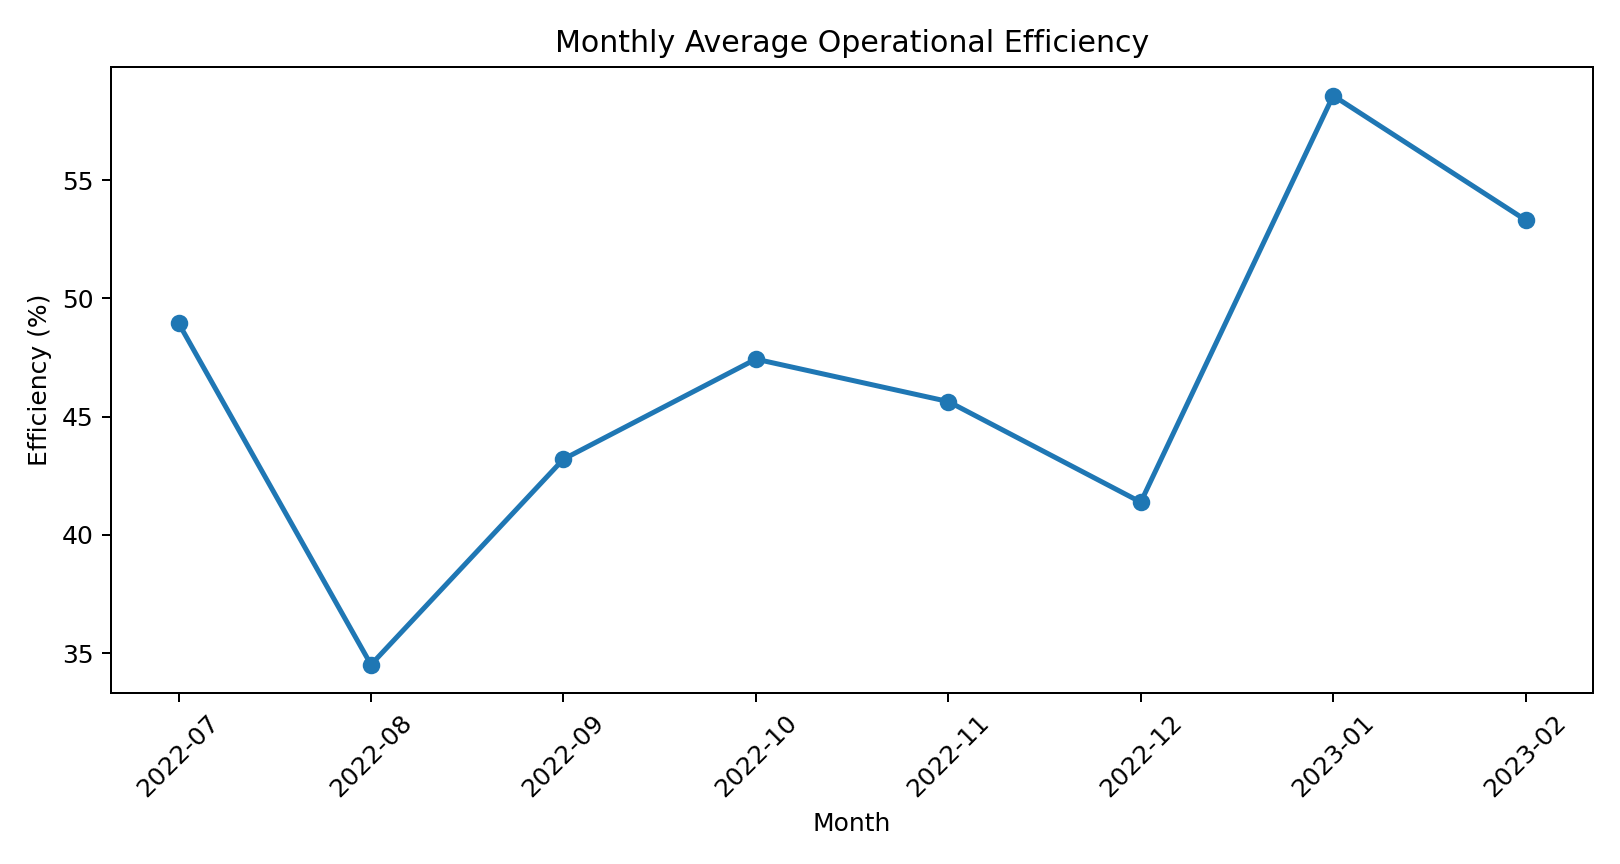
\includegraphics[width=0.92\textwidth]{outputs/monthly_efficiency.png}
\caption{Monthly average operational efficiency from the real bottling-line dataset.}
\end{figure}

The monthly efficiency chart shows considerable variation across the study period. Lower performance is visible in August 2022 and December 2022, while stronger operational performance appears in January 2023. This confirms that the line does not behave like a stable deterministic production system; instead, it experiences substantial variability that justifies simulation-based evaluation.

\subsection{Downtime Structure}
The downtime-event distribution is strongly right-skewed. The median event duration is 1.50 minutes, the 90th percentile is 6.50 minutes, the 95th percentile is 13.74 minutes, and the maximum observed event is 349.83 minutes. These statistics indicate that the line experiences many short interruptions but also a small number of very large disruptions.

\begin{figure}[H]
\centering
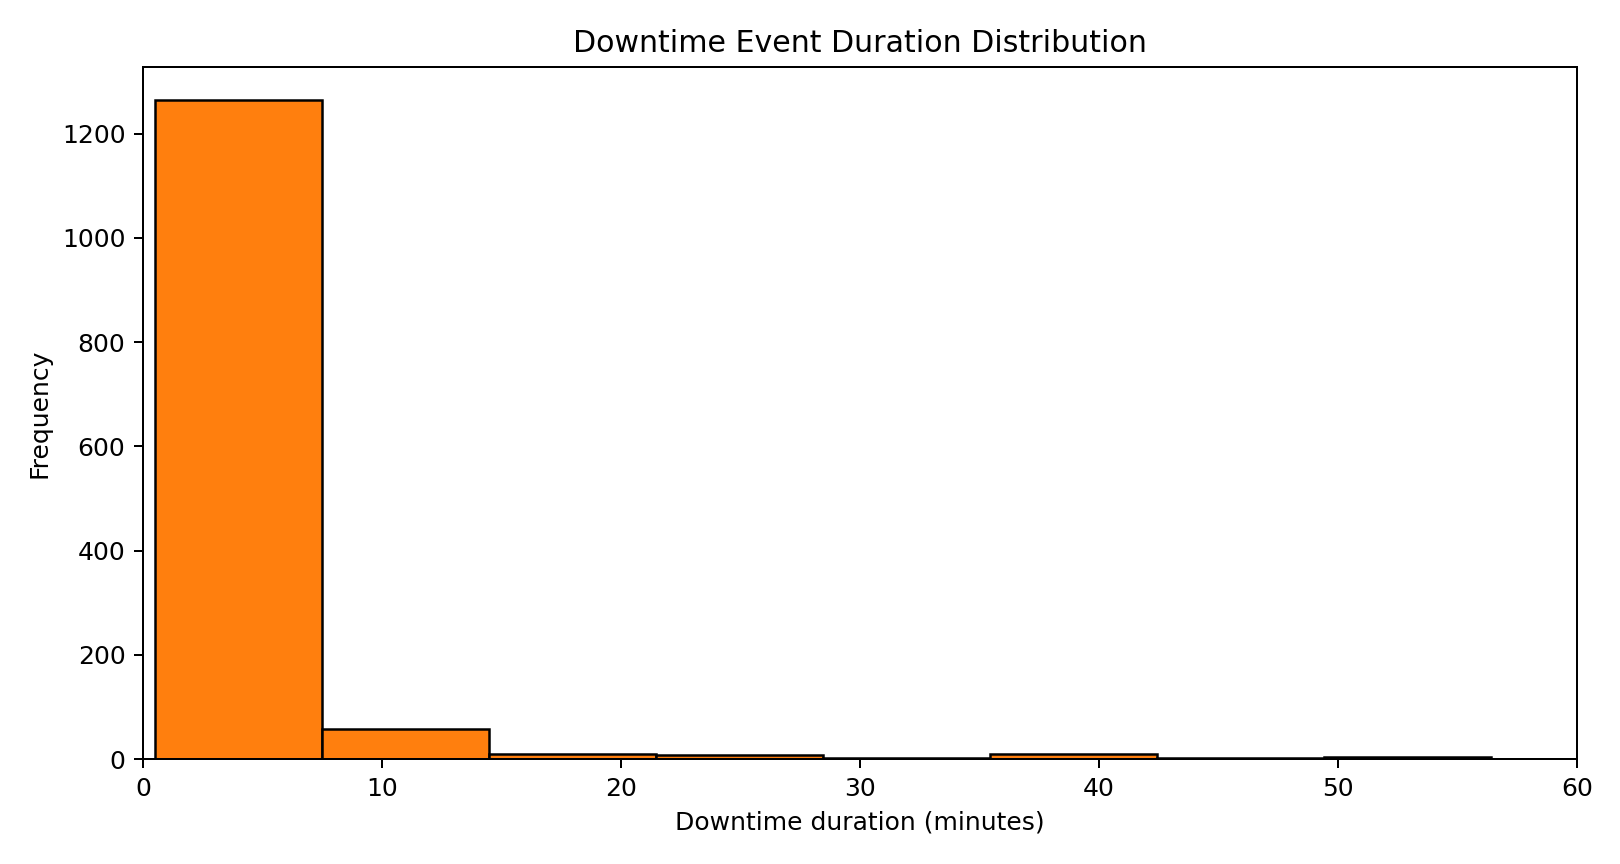
\includegraphics[width=0.92\textwidth]{outputs/downtime_distribution.png}
\caption{Distribution of downtime-event duration, truncated at 60 minutes for readability.}
\end{figure}

\begin{table}[H]
\centering
\caption{Downtime Category Structure}
\begin{tabular}{lrr}
\toprule
\textbf{Category} & \textbf{Event Count} & \textbf{Share of Downtime Minutes} \\
\midrule
Micro ($\leq$ 2 min) & 851 & 13.59\% \\
Minor (2--10 min) & 443 & 20.15\% \\
Major ($>$ 10 min) & 94 & 66.26\% \\
\bottomrule
\end{tabular}
\end{table}

\begin{figure}[H]
\centering
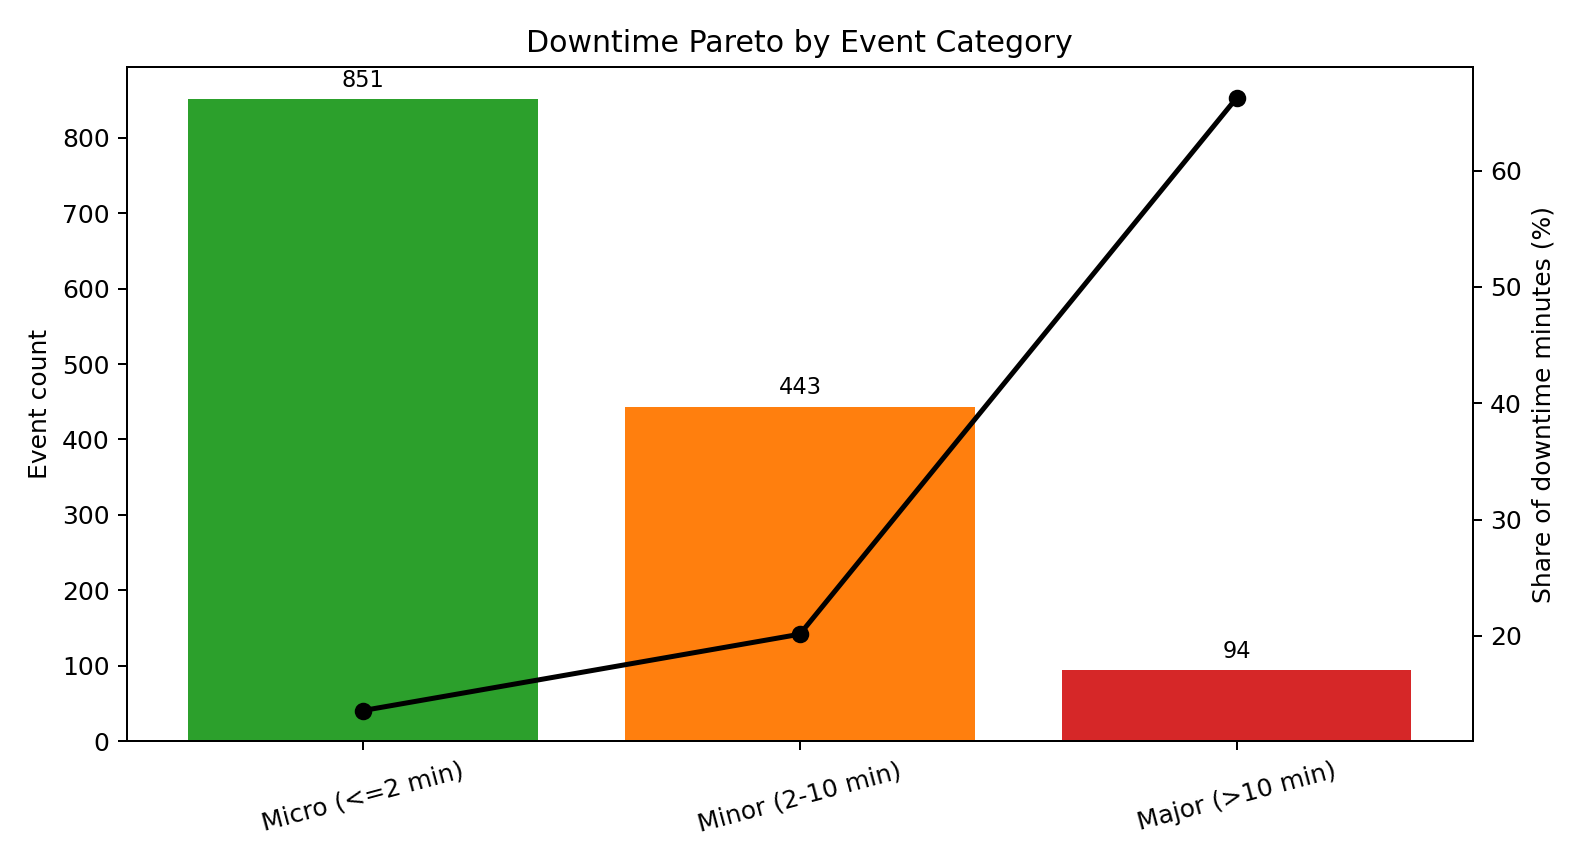
\includegraphics[width=0.92\textwidth]{outputs/downtime_category_pareto.png}
\caption{Downtime Pareto by event category. Major stoppages are rare but dominant in lost time.}
\end{figure}

The downtime Pareto view provides one of the most important insights of the paper. Micro-stoppages account for 61.31\% of all events but only 13.59\% of total downtime minutes, whereas major stoppages represent only 6.77\% of events but consume 66.26\% of lost time. This means that event frequency alone does not identify the highest productivity loss. Lean prioritization must be based on lost-time severity.

\subsection{Pause Time and Efficiency Relationship}
At the date-aggregated level, pause time showed a strong negative correlation with efficiency ($r=-0.707$). This means that as daily pause time increases, effective operating efficiency falls sharply.

\begin{figure}[H]
\centering
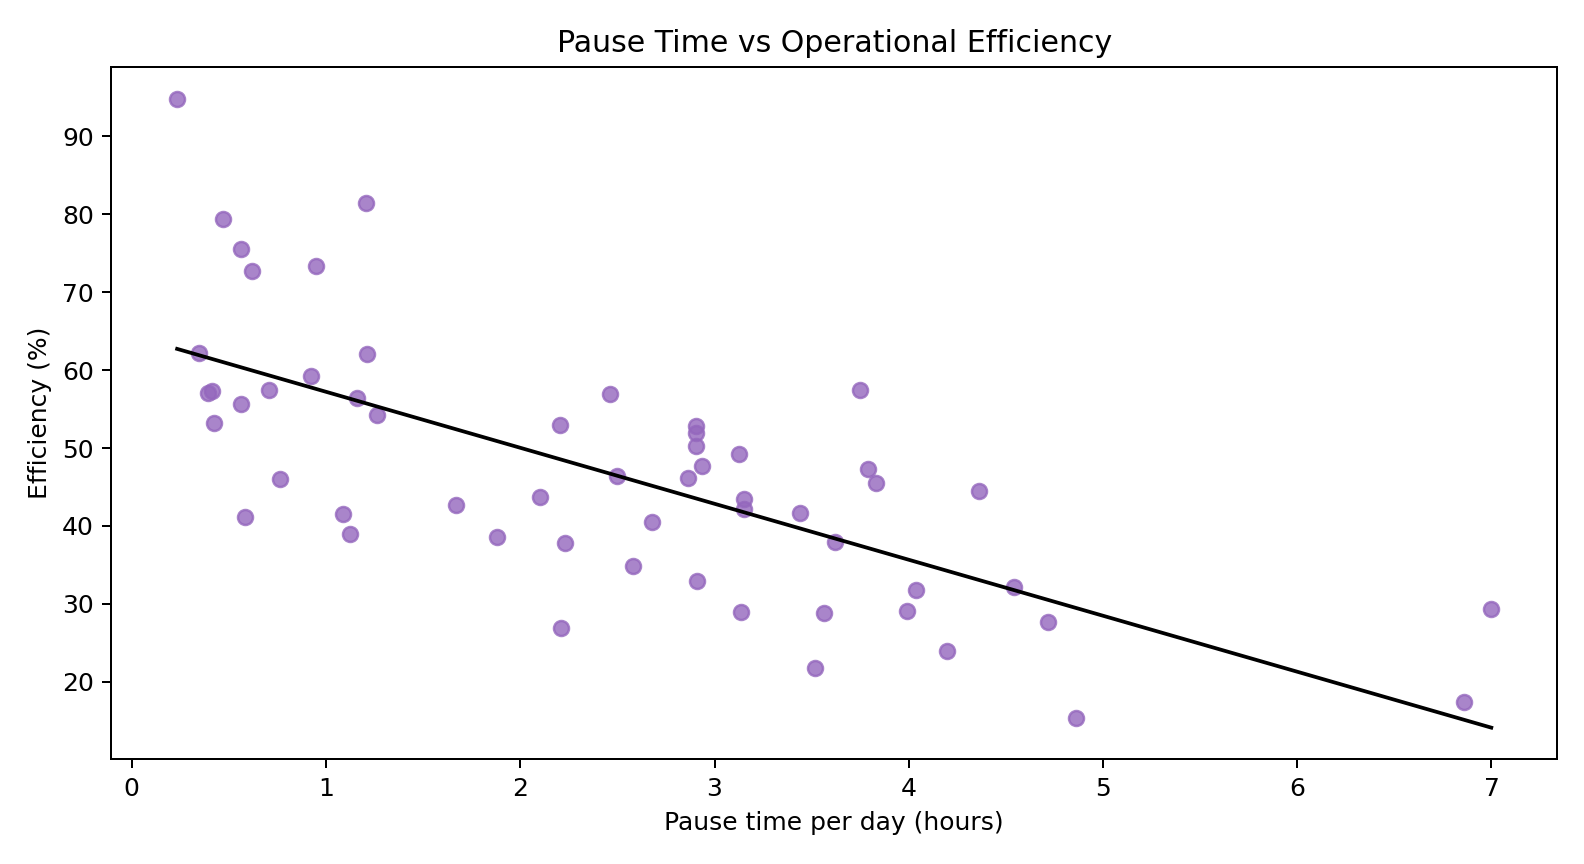
\includegraphics[width=0.92\textwidth]{outputs/pause_vs_efficiency.png}
\caption{Daily pause time versus operational efficiency.}
\end{figure}

The scatter plot shows a clear downward trend. This provides further evidence that reducing downtime is the most direct productivity-improvement lever in the observed system.

\subsection{Production Rate by Product Type}
The production-rate comparison by product size is shown below.

\begin{figure}[H]
\centering
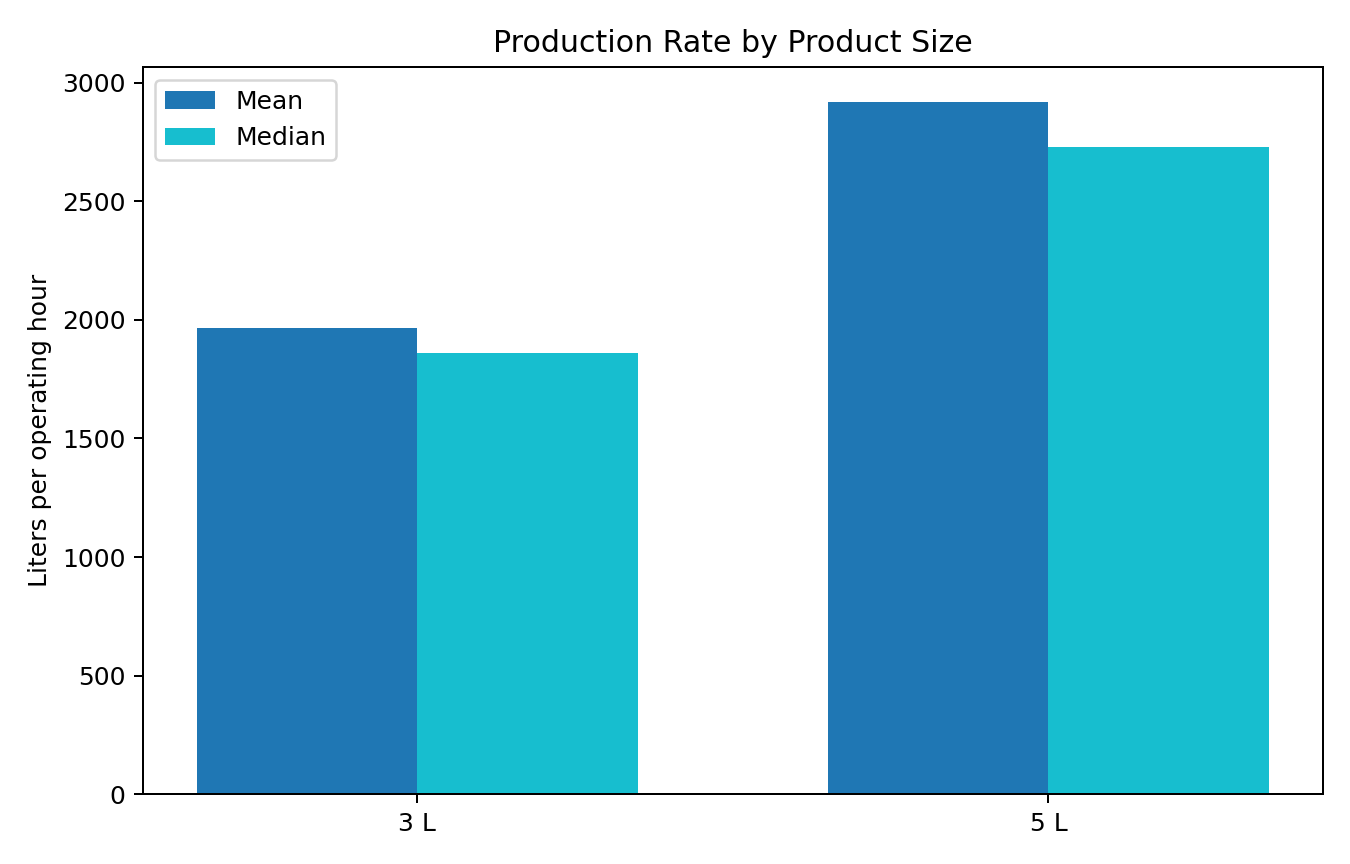
\includegraphics[width=0.85\textwidth]{outputs/product_rate_comparison.png}
\caption{Mean and median production rate by product size.}
\end{figure}

The 5-liter product has both higher mean and higher median production rate than the 3-liter product. This suggests that product mix can also influence line performance and may become an additional decision variable in future scheduling or line-balancing studies.

\subsection{Simulation Results}
The simulation baseline produced 211,924.69 liters on average across the resampled production horizon. This closely matches the observed output of the real system, indicating that the simulation reasonably preserves actual operating behavior.

\begin{table}[H]
\centering
\caption{Simulation Results for Lean Scenarios}
\begin{tabular}{lrrrr}
\toprule
\textbf{Scenario} & \textbf{Mean Output (L)} & \textbf{Gain (\%)} & \textbf{Efficiency (\%)} & \textbf{Eff. Gain (pp)} \\
\midrule
Baseline & 211,924.69 & 0.00 & 42.37 & 0.00 \\
5S + Visual Management & 216,866.69 & 2.33 & 43.25 & 0.88 \\
TPM & 255,604.10 & 20.61 & 50.81 & 8.44 \\
Integrated Lean Bundle & 280,142.22 & 32.19 & 55.33 & 12.96 \\
\bottomrule
\end{tabular}
\end{table}

\begin{table}[H]
\centering
\caption{Simulation Uncertainty Range}
\begin{tabular}{lrr}
\toprule
\textbf{Scenario} & \textbf{P05 Output (L)} & \textbf{P95 Output (L)} \\
\midrule
Baseline & 188,572.81 & 236,799.79 \\
5S + Visual Management & 192,906.87 & 242,100.46 \\
TPM & 226,295.58 & 287,389.24 \\
Integrated Lean Bundle & 247,828.10 & 314,804.33 \\
\bottomrule
\end{tabular}
\end{table}

\begin{figure}[H]
\centering
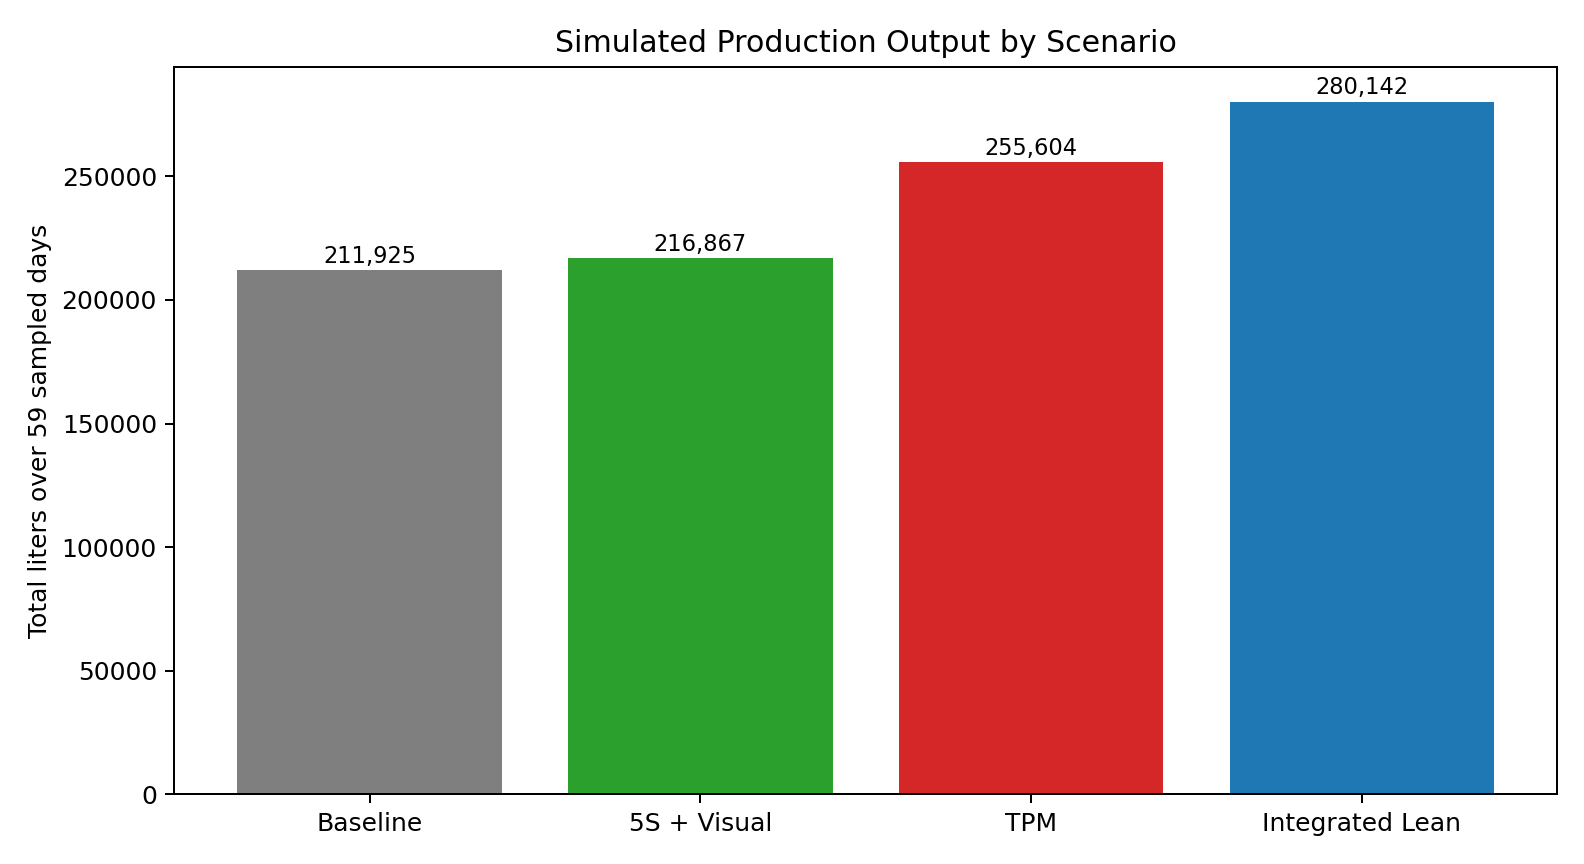
\includegraphics[width=0.92\textwidth]{outputs/scenario_output.png}
\caption{Mean simulated production output across the baseline and lean scenarios.}
\end{figure}

The simulation results show that 5S and visual management provide only a modest output gain of 2.33\%. This is because the scenario mainly targets micro-stoppages, which are frequent but contribute relatively little to total lost time. By contrast, TPM produces a much larger gain of 20.61\% because it directly targets major stoppages, which dominate downtime minutes. The integrated lean bundle produces the highest gain, improving output by 32.19\% and raising simulated availability from 42.37\% to 55.33\%.

\section{Discussion}
The results strongly suggest that lean implementation should be based on the structure of operational loss rather than on the visibility or frequency of events alone. In many production systems, micro-stoppages attract attention because they happen often and disrupt workflow visibly. However, as demonstrated in this study, those frequent interruptions may not be the dominant cause of lost production.

For the bottling line studied here, major stoppages are the real productivity driver. Although they are relatively rare, they consume most of the downtime minutes. This explains why TPM, which focuses on equipment reliability and breakdown reduction, produces far more improvement than 5S alone. The result is fully consistent with the broader lean-simulation literature, which emphasizes context-specific tool selection [4], [5].

Another important implication is the role of digital manufacturing data in strengthening lean analysis. Instead of relying only on static value stream mapping or qualitative observation, this study uses event-level downtime records and simulation. This is aligned with the direction suggested by smart manufacturing and digital twin research [6], [10]. The practical value is clear: real data allow the analyst to identify high-leverage interventions rather than applying lean tools generically.

For final-year engineering research, this approach is especially useful because it combines core industrial engineering ideas: data analysis, productivity evaluation, lean manufacturing, operations research thinking, and simulation-based decision support. It also produces a study that is more rigorous than a purely descriptive case report.

\section{Implementation Recommendations}
Based on the results, the recommended order of lean implementation is:
\begin{enumerate}
    \item \textbf{First priority: TPM.} The plant should focus on reducing long-duration stoppages through maintenance planning, preventive checks, fast fault recovery, and equipment reliability tracking.
    \item \textbf{Second priority: 5S and visual management.} These tools should be used to reduce small disruptions, improve operator control, and standardize the workplace.
    \item \textbf{Third priority: integrated lean bundle.} Once maintenance discipline is improved, the plant can combine TPM with micro-stop reduction and standard work for broader gains.
\end{enumerate}

\begin{table}[H]
\centering
\caption{Recommended Lean Implementation Roadmap}
\begin{tabular}{p{3cm}p{4.2cm}p{7cm}}
\toprule
\textbf{Priority} & \textbf{Lean Focus} & \textbf{Expected Impact} \\
\midrule
1 & TPM and maintenance discipline & Highest reduction in lost-time severity by targeting major stoppages. \\
2 & 5S and visual management & Better workplace organization and reduction in frequent micro-disruptions. \\
3 & Integrated lean bundle & Combined gains from reliability, stabilization, and standardized work. \\
\bottomrule
\end{tabular}
\end{table}

\section{Conclusion}
This paper presented a self-contained, one-column research study on simulation-based lean manufacturing using a real industrial beverage bottling dataset. The study showed that the system suffers from low availability, high downtime, and substantial variability over time. Although micro-stoppages are the most frequent events, major stoppages dominate lost production time.

The simulation results demonstrated that:
\begin{enumerate}
    \item 5S and visual management improve output by 2.33\%;
    \item TPM improves output by 20.61\%;
    \item an integrated lean bundle improves output by 32.19\% and raises simulated availability from 42.37\% to 55.33\%.
\end{enumerate}

The main managerial conclusion is that maintenance-led reduction of major stoppages should be prioritized first. The main academic contribution is the development of a reproducible, open-data framework for simulation-based lean research suitable for student projects, SME analysis, and future applied manufacturing studies.

\section{Limitations and Future Scope}
This study has three major limitations. First, the lean scenarios are simulated assumptions rather than observed post-implementation outcomes. Second, the dataset does not contain detailed cause-coded downtime labels, so the mapping from downtime category to lean tool remains inferential. Third, the analysis is based on one industrial case, so the results should not be generalized mechanically to all production systems.

Future work can improve the present study by collecting root-cause-coded downtime data, operator-level observations, quality-loss information, and real post-intervention performance records. Future studies may also extend the simulation to include changeover analysis, workforce allocation, line balancing, and cost-benefit evaluation.

\section*{Acknowledgement}
The authors sincerely acknowledge the guidance and support of \textbf{Dr.\ MOHD SHUAIB} from the \textbf{Mechanical Department}. His academic guidance was valuable in shaping the direction and structure of this work.

\begin{thebibliography}{11}

\bibitem{r1}
I. Belekoukias, J. A. Garza-Reyes, and V. Kumar, ``The impact of lean methods and tools on the operational performance of manufacturing organisations,'' \emph{International Journal of Production Research}, vol. 52, no. 18, pp. 5346--5366, 2014, doi: 10.1080/00207543.2014.903348.

\bibitem{r2}
O. Oleghe and K. Salonitis, ``Hybrid simulation modelling of the human-production process interface in lean manufacturing systems,'' \emph{International Journal of Lean Six Sigma}, vol. 10, no. 2, pp. 665--690, 2019, doi: 10.1108/IJLSS-01-2018-0004.

\bibitem{r3}
F. Yu and Z. Chen, ``Tools, application areas and challenges of factory simulation in Small and Medium-Sized Enterprises -- A Review,'' \emph{Procedia CIRP}, vol. 104, pp. 399--404, 2021, doi: 10.1016/j.procir.2021.11.067.

\bibitem{r4}
J. Possik, A. Zouggar-Amrani, B. Vallespir, and G. Zacharewicz, ``Lean techniques impact evaluation methodology based on a co-simulation framework for manufacturing systems,'' \emph{International Journal of Computer Integrated Manufacturing}, vol. 35, no. 1, pp. 91--111, 2022, doi: 10.1080/0951192X.2021.1972468.

\bibitem{r5}
S. Frecassetti, B. Kassem, K. Kundu, M. Ferrazzi, and A. Portioli-Staudacher, ``Introducing Lean practices through simulation: A case study in an Italian SME,'' \emph{Quality Management Journal}, vol. 30, no. 2, pp. 90--104, 2023, doi: 10.1080/10686967.2023.2171326.

\bibitem{r6}
J. A. C. Bokhorst, W. Knol, J. Slomp, and T. Bortolotti, ``Assessing to what extent smart manufacturing builds on lean principles,'' \emph{International Journal of Production Economics}, vol. 253, art. no. 108599, 2022, doi: 10.1016/j.ijpe.2022.108599.

\bibitem{r7}
G. A. David, P. M. C. Monson, C. Soares Junior, P. O. Concei\c{c}\~ao Junior, P. R. Aguiar, and A. Simeone, ``IoT-Driven Deep Learning for Enhanced Industrial Production Forecasting,'' \emph{IEEE Internet of Things Journal}, vol. 11, no. 23, pp. 38486--38495, 2024, doi: 10.1109/JIOT.2024.3447579.

\bibitem{r8}
G. A. David, P. M. C. Monson, and C. Soares Junior, \emph{Industrial Production Time-Series Dataset from a Beverage Bottling Line}. Zenodo, Jan. 4, 2026. doi: 10.5281/zenodo.18146866.

\bibitem{r9}
J. M. Matindana and M. J. Shoshiwa, ``Lean manufacturing implementation in food and beverage SMEs in Tanzania: using structural equation modelling (SEM),'' \emph{Management System Engineering}, vol. 4, no. 1, pp. 1--14, 2025, doi: 10.1007/s44176-025-00036-3.

\bibitem{r10}
M. Reslan, M. J. Triebe, R. Venketesh, and A. J. Hartwell, ``Automation of Value Stream Mapping: A Case Study on Enhancing Lean Manufacturing Tools Through Digital Twins,'' \emph{Procedia CIRP}, vol. 134, pp. 455--460, 2025, doi: 10.1016/j.procir.2025.02.159.

\bibitem{r11}
C. Unal and S. Bilget, ``Examination of lean manufacturing systems by simulation technique in apparel industry,'' \emph{The Journal of The Textile Institute}, vol. 112, no. 3, pp. 377--387, 2021, doi: 10.1080/00405000.2020.1756104.

\end{thebibliography}

\end{document}
